\documentclass[landscape]{slides}

\usepackage{animate}
\usepackage[landscape]{geometry}
\usepackage[utf8]{inputenc}
\usepackage{pstricks}
\usepackage{graphicx}
\usepackage{graphics}
\usepackage{color}
\usepackage{amsmath}
\usepackage{amsfonts}
\usepackage{amsthm}
\usepackage{amssymb}
\usepackage{wasysym}
\usepackage{pgf, tikz}
\usetikzlibrary{decorations.markings}
\usetikzlibrary{math}

\setlength{\textwidth}{25.0cm}
\setlength{\textheight}{19.0cm}
\setlength{\oddsidemargin}{-1.6cm}
\setlength{\evensidemargin}{-1.6cm}
\setlength{\topmargin}{-2.4cm}

\begin{document}

% ____________________________________________________________________________
\begin{slide}
\thispagestyle{empty}

\begin{center}
\textbf{\Large Laboratory investigiton of reconnection \\[0.4cm] weakened by a guide field}

\vspace{3.0cm}

\textrm{\large S. Bolanos$^{\star}$, A. Sladkov$^{\dagger}$, \underline{R. SMETS}$^{\dagger}$, J. Fuchs$^{\star}$, et al.}
\end{center}

\vspace{1.0cm}

$^{\dagger}$LPP, $^{\star}$LULI

\vspace{2.0cm}

\textit{\large "Lab7 meeting", 21 december 2022}

\end{slide}

% ____________________________________________________________________________
\begin{slide}
\large{\textbf{2D Magnetic reconnection}}


\vspace{1.0cm}

\begin{center}
\begin{tikzpicture}

\node[inner sep=0pt] (disk) at (0,0)
    {\includegraphics[width=.8\textwidth]{sweet.png}};

\node at ( 4.0, 1.6) {$L$} ;
\node at (-3.6,-0.2) {$\delta$} ;

\node at ( 2.0, 3.4) {$U$} ;
\node at ( 1.0, 3.0) {$\downarrow$} ;
\node at (-7.0, 0.6) {$v$} ;
\node at (-7.0,-0.2) {$\longleftarrow$} ;

\node at (-5.0, 3.0) {$B_0$} ;
\node at ( 3.8, 0.4) {$\sigma \neq 0$} ;


%\node at (-1.0, 1.2) {$\longleftarrow$} ;
%\node at (-1.0,-1.4) {$\longrightarrow$} ;

\node at (-1.0,-2.2) {$\odot$} ;
\node at (-1.0,-3.2) {Reconnection Electric Field} ;

\end{tikzpicture}
\end{center}



$\rightarrow$ converts magnetic energy into kinetic energy \\[0.0cm]
$\bullet$ we rarely observe reconnection, but the consequences...

\end{slide}

% ____________________________________________________________________________
\begin{slide}
\large{\textbf{Fast Reconnection \& Hall effect} [Birn et al., JGR 2001]}

\begin{tikzpicture}[scale=0.5]

\def\shift{+3.0}
\def\dyb{1.6}
\def\eta{6.0}
\def\aa{1.0}
\def\bb{1.0}
\def\xmax{+8.}

\def\xbza{2.0}
\def\ybza{0.95}
\def\xbzb{6.0}
\def\ybzb{1.6}

\def\dyja{1.3}
\def\dyjb{0.6}
\def\zeta{6.0}
\def\shiftja{+3.0}
\def\shiftjb{+3.4}
\def\xmaxj{+7.}
\def\xminj{+1.}

\def\xea{+7.0}
\def\yea{+2.8}
\def\xeb{+7.6}
\def\yeb{+2.0}

\def\xec{0.2*\shift}
\def\yec{0.4*\dyb}

\tikzset{declare function={bline_tl(\x)=+\dyb-\eta*\bb+\bb*sqrt(\eta*\eta+((-\x-\shift)/\aa)^2);}}
\tikzset{declare function={bline_tr(\x)=+\dyb-\eta*\bb+\bb*sqrt(\eta*\eta+((+\x-\shift)/\aa)^2);}}
\tikzset{declare function={bline_bl(\x)=-\dyb+\eta*\bb-\bb*sqrt(\eta*\eta+((-\x-\shift)/\aa)^2);}}
\tikzset{declare function={bline_br(\x)=-\dyb+\eta*\bb-\bb*sqrt(\eta*\eta+((+\x-\shift)/\aa)^2);}}

\tikzset{arrowplus/.pic = {\draw[very thick] (0, 0) circle (3pt);
                           \draw[very thick] (0, 0) circle (0.5pt); }
        }

\tikzset{arrowminus/.pic = {\draw[very thick] (0, 0) circle (3pt);
                            \draw[very thick] ( 0.0,-0.1) -- ( 0.0,+0.1);
                            \draw[very thick] (-0.1, 0.0) -- (+0.1, 0.0);}
        }

\tikzset{declare function={jlinea_tl(\x)=+\dyja-\zeta*\bb+\bb*sqrt(\zeta*\eta+((-\x-\shiftja)/\aa)^2);}}
\tikzset{declare function={jlineb_tl(\x)=+\dyjb-\zeta*\bb+\bb*sqrt(\zeta*\eta+((-\x-\shiftjb)/\aa)^2);}}
\tikzset{declare function={jlinea_tr(\x)=+\dyja-\zeta*\bb+\bb*sqrt(\zeta*\eta+((+\x-\shiftja)/\aa)^2);}}
\tikzset{declare function={jlineb_tr(\x)=+\dyjb-\zeta*\bb+\bb*sqrt(\zeta*\eta+((+\x-\shiftjb)/\aa)^2);}}
\tikzset{declare function={jlinea_bl(\x)=-\dyja+\zeta*\bb-\bb*sqrt(\zeta*\eta+((-\x-\shiftja)/\aa)^2);}}
\tikzset{declare function={jlineb_bl(\x)=-\dyjb+\zeta*\bb-\bb*sqrt(\zeta*\eta+((-\x-\shiftjb)/\aa)^2);}}
\tikzset{declare function={jlinea_br(\x)=-\dyja+\zeta*\bb-\bb*sqrt(\zeta*\eta+((+\x-\shiftja)/\aa)^2);}}
\tikzset{declare function={jlineb_br(\x)=-\dyjb+\zeta*\bb-\bb*sqrt(\zeta*\eta+((+\x-\shiftjb)/\aa)^2);}}

\tikzset{frame/.pic = {\draw[very thick, ->] (0.0, 0.0) -- ( 0.5, 0.0);
                       \node at ( 0.7, 0.0) {$x$};
                       \draw[very thick, ->] (0.0, 0.0) -- ( 0.0, 0.5);
                       \node at ( 0.0, 0.7) {$y$};
                       \draw[very thick, ->] (0.0, 0.0) -- (-0.4,-0.4);
                       \node at (-0.6,-0.6) {$z$};}
        }

%B field in xy plane
\draw[very thick, olive,   -] (-\shift, \dyb) -- (0, \dyb);
\draw [domain=-\xmax:-\shift, very thick, olive,  -] plot(\x, {bline_tl(\x)});

\draw[very thick, olive,  ->] (\shift, \dyb) -- (0, \dyb);
\draw [domain=\shift:\xmax, very thick, olive,  -] plot(\x, {bline_tr(\x)});

\draw[very thick, olive,  ->] (-\shift, -\dyb) -- (0, -\dyb);
\draw [domain=-\xmax:-\shift, very thick, olive,  -] plot(\x, {bline_bl(\x)});

\draw[very thick, olive,   -] (\shift, -\dyb) -- (0, -\dyb);
\draw [domain=\shift:\xmax, very thick, olive,  -] plot(\x, {bline_br(\x)});

%B field along z
\path[very thick, olive] (-\xbza,+\ybza) pic{arrowplus};
\path[very thick, olive] (+\xbza,+\ybza) pic{arrowminus};
\path[very thick, olive] (-\xbza,-\ybza) pic{arrowminus};
\path[very thick, olive] (+\xbza,-\ybza) pic{arrowplus};

\path[very thick, olive] (-\xbzb,+\ybzb) pic{arrowplus};
\path[very thick, olive] (+\xbzb,+\ybzb) pic{arrowminus};
\path[very thick, olive] (-\xbzb,-\ybzb) pic{arrowminus};
\path[very thick, olive] (+\xbzb,-\ybzb) pic{arrowplus};

%J field in xy plane
\draw [domain=-\xmaxj:-\shift, very thick, black,  -] plot(\x, {jlinea_tl(\x)});
\draw [very thick, black,  ->] (-\xminj,  \dyja) -- (-\shift, \dyja);
\draw [domain=-\shift:-\xmaxj, very thick, black, <-] plot(\x, {jlineb_tl(\x)});
\draw [very thick, black,   -] (-\shift,  \dyjb) -- (-\xminj,  \dyjb);

\draw [domain= \xmaxj: \shift, very thick, black,  -] plot(\x, {jlinea_tr(\x)});
\draw [very thick, black,  ->] ( \xminj,  \dyja) -- ( \shift, \dyja);
\draw [domain= \shift: \xmaxj, very thick, black, <-] plot(\x, {jlineb_tr(\x)});
\draw [very thick, black,   -] ( \shift,  \dyjb) -- ( \xminj,  \dyjb);

\draw [domain=-\xmaxj:-\shift, very thick, black,  -] plot(\x, {jlinea_bl(\x)});
\draw [very thick, black,  ->] (-\xminj,-\dyja) -- (-\shift, -\dyja);
\draw [domain=-\shift:-\xmaxj, very thick, black, <-] plot(\x, {jlineb_bl(\x)});
\draw [very thick, black,   -] (-\shift, -\dyjb) -- (-\xminj, -\dyjb);

\draw [domain= \xmaxj: \shift, very thick, black,  -] plot(\x, {jlinea_br(\x)});
\draw [very thick, black,  ->] ( \xminj, -\dyja) -- ( \shift, -\dyja);
\draw [domain= \shift: \xmaxj, very thick, black, <-] plot(\x, {jlineb_br(\x)});
\draw [very thick, black,   -] ( \shift, -\dyjb) -- ( \xminj, -\dyjb);

%J field along z
\path[very thick, black] (-5, 0) pic{arrowplus};
\path[very thick, black] (-3, 0) pic{arrowplus};
\path[very thick, black] (-1, 0) pic{arrowplus};
\path[very thick, black] ( 1, 0) pic{arrowplus};
\path[very thick, black] ( 3, 0) pic{arrowplus};
\path[very thick, black] ( 5, 0) pic{arrowplus};

%E field in the XY plane
\draw [very thick, brown, ->] (-\xea, \yea) -- (-\xeb, \yeb);
\draw [very thick, brown, ->] ( \xea, \yea) -- ( \xeb, \yeb);
\draw [very thick, brown, ->] (-\xea,-\yea) -- (-\xeb,-\yeb);
\draw [very thick, brown, ->] ( \xea,-\yea) -- ( \xeb,-\yeb);

\draw [very thick, brown, ->] (-\xec, \dyb) -- (-\xec, \yec);
\draw [very thick, brown, ->] ( \xec, \dyb) -- ( \xec, \yec);
\draw [very thick, brown, ->] (-\xec,-\dyb) -- (-\xec,-\yec);
\draw [very thick, brown, ->] ( \xec,-\dyb) -- ( \xec,-\yec);

%J field along z
\path[very thick, brown] (-7, 0) pic{arrowminus};
\path[very thick, brown] ( 7, 0) pic{arrowminus};

\node[olive] at ( 6.3, 3.4) {$B$-field};
\node[black] at (-7.6, 1.0) {$J$-field};
\node[brown] at ( 7.2,-0.6) {$E$-field};

% axis
\path[very thick] (0.0,3.5) pic{frame};

\end{tikzpicture}


\begin{tabular}{lcl}
Ideal MHD & : & $\mathbf E = - \mathbf U \times \mathbf B$ \\[0.4cm]
$p^+$ Diff. region & : & $\mathbf E = (\mathbf J \times \mathbf B) / en$ \\[0.4cm]
$e^-$ Diff. region & : & $\mathbf E = - \boldsymbol{\nabla} . \; \mathbf P_e / en$
\end{tabular}

\end{slide}

% ____________________________________________________________________________
\begin{slide}
\large{\textbf{Planetary Magnetospheres} [Dungey, PRL 1961]}


\vspace{1.0cm}

\begin{center}
\begin{tikzpicture}

\node[inner sep=0pt] (disk) at (0,0)
    {\includegraphics[width=.8\textwidth]{magnetosphere.png}};

\node (A) at (-2.0, 4.4) {$_\leftarrow$ To the Sun} ;
\node (B) at (-8.4, 4.0) {IMF} ;
\node (C) at ( 4.0,-3.0) {Planetary Magnetic Field} ;

\end{tikzpicture}
\end{center}



At day-side Magnetopause \& in the Magnetotail\\
$\rightarrow$ $\beta \sim 1$, $L \rightarrow \infty$, $\gamma \sim 1$

\end{slide}

% ____________________________________________________________________________
\begin{slide}
\large{\textbf{Solar prominence merging} [Aulanier et al., ApJ 2005]}


\vspace{1.0cm}

\begin{center}
\begin{tikzpicture}

\node[inner sep=0pt] (disk) at (0,0)
    {\includegraphics[width=.7\textwidth]{flare.png}};

\node (A) at (-2.4,-1.6) {-} ;
\node (B) at ( 5.4,-2.0) {-} ;
\node (C) at ( 0.0, 0.6) {+} ;
\node (D) at ( 6.6,-0.2) {+} ;

\end{tikzpicture}
\end{center}



Cold dense tube in hot tenuous coronna, highly 3D\\
$\rightarrow$ $\beta \sim 10^{-2}$, $L \rightarrow \infty$, $\gamma \sim 1$

\end{slide}

% ____________________________________________________________________________
\begin{slide}
\large{\textbf{Striped pulsar wind} [Bogovalov, A\&A 1999]}


\vspace{1.0cm}

\begin{center}
\begin{tikzpicture}

\node[inner sep=0pt] (disk) at (0,0)
    {\includegraphics[width=.8\textwidth]{pulsar.png}};

\node at ( 5.6, 3.9) {$\otimes$} ;
\node at ( 1.6, 3.0) {$\otimes$} ;
\node at (-2.4, 2.0) {$\otimes$} ;
\node at (-2.4,-3.0) {$\odot$} ;
\node at ( 1.6,-3.3) {$\odot$} ;
\node at ( 5.6,-3.8) {$\odot$} ;

\node at (-4.0,-0.8) {$\odot$} ;
\node at (-1.8,-0.4) {$\otimes$} ;
\node at ( 1.0,-0.2) {$\odot$} ;
\node at ( 4.0, 0.0) {$\otimes$} ;
\node at ( 6.6, 0.2) {$\odot$} ;

\node at (-6.4, 2.6) {$\boldsymbol{\Omega}$} ;
\node at (-8.6, 3.0) {$\boldsymbol{\mu}$} ;

\end{tikzpicture}
\end{center}



Shock-driven reconnection in a pair-plasmas\\
$\rightarrow$ $\sigma \sim 10^4$, $L \rightarrow \infty$, $\gamma \sim 10^3$\\
$\rightarrow$ EM energy to synchrotron emmitting electrons (X \& $\gamma$)

\end{slide}

% ____________________________________________________________________________
\begin{slide}
\large{\textbf{Microquasar} [de Gouveia dal Pino \& Lazarian, A\&A 2005]}


\vspace{1.0cm}

\begin{center}
\begin{tikzpicture}

\node[inner sep=0pt] (disk) at (0,0)
    {\includegraphics[width=.6\textwidth]{disk.png}};

\node at (-10.0,-1.0) {Compact} ;
\node at (-10.0,-2.0) {Object} ;
\node at ( 5.0,-1.0) {disk} ;

\end{tikzpicture}
\end{center}

 % magneto-centrifugal acceleration

Can explain the steep power-law state of photons\\
$\rightarrow$ $\beta \leq 1$, $L \rightarrow \infty$, $\gamma \gg 1$\\

\end{slide}

%%% % ____________________________________________________________________________
%%% \begin{slide}
%%% \large{\textbf{$\boldsymbol{\gamma}$ ray bursts (Fireball model) } [Thompson, 1994]}
%%% 
%%% 
\vspace{1.0cm}

\begin{center}
\begin{tikzpicture}

\node[inner sep=0pt] (disk) at (0,0)
    {\includegraphics[width=.8\textwidth]{fireball.png}};

\node at (-8.0, 2.6) {$10^{+46}$ J} ;

\node at (-3.0, 3.0) {Pre-Burst} ; % thermal
\node at ( 1.4, 2.0) {Burst} ;
\node at ( 6.6,-2.0) {Afterglow} ;
\node at (11.0, 2.0) {IGM} ;

\node at (-0.4, 1.0) {$\photon$} ;
\node at (-0.4, 0.0) {$\gamma$} ;

\node at ( 5.0, 2.0) {$\photon$} ;
\node at ( 5.0, 1.0) {$\photon$} ;
\node at ( 5.0, 0.0) {$\gamma$} ;
\node at ( 5.0,-1.0) {$\photon$} ;

\node at (12.0, 0.0) {$\photon$} ;
\node at (12.0,-1.0) {X $\rightarrow$ radio} ;
\node at (12.0,-2.0) {$\photon$} ;

\end{tikzpicture}
\end{center}

 % compact merger or collapsar
%%% 
%%% Ultra-relativistic with $\beta \leq 10^{-4}$ $\rightarrow$ $f(\gamma) \propto \gamma^{-\delta}$ with $p \sim -2.2$\\
%%% $\rightarrow$ Associated $\delta \sim -1.6$ for synchrotron photons
%%% 
%%% \end{slide}

% ____________________________________________________________________________
\begin{slide}
\large{\textbf{With high-intensity Lasers...} [Nielson et al., 2006]}


\vspace{1.0cm}

\begin{center}
\begin{tikzpicture}

\node[inner sep=0pt] (disk) at (0,0)
    {\includegraphics[width=.7\textwidth]{planar.png}};

\node at ( 3.4, 4.4) {$\boldsymbol{\nabla} n$} ;
\node at ( 3.4, 3.4) {$\downarrow$} ;

\node at (-0.4, 2.4) {$\swarrow$} ;
\node at ( 1.0, 2.4) {$\boldsymbol{\nabla} T_e$} ;

\end{tikzpicture}
\end{center}



$\bullet$ Two closeby hotspots on solid target :\\
$\rightarrow$ 2 magnetic loops created by Biermann-Battery effect\\
$\rightarrow$ newly created magnetic flux expeled by reconnection

\end{slide}

% ____________________________________________________________________________
\begin{slide}
\large{\textbf{Importance of Hall effect for fast reconnection}}

\begin{center}
\includegraphics[width=0.7\textwidth]{scheme.jpg}
\end{center}

$\bullet$ (Hall) $E_{XY}$ electric field associated to $J_Z$ and $B_{XY}$\\
$\bullet$ $J_Z$ grows at the tip of each loops when colliding\\
$\rightarrow$ quadrupolar $B_Z$ grows because $E_{XY}$ is no more curl-free\\
$\bullet$ $J_{XY}$ associated to this out-of-plane magnetic field\\
$\rightarrow$ carried by electrons because protons are demagnetized

\end{slide}

% ____________________________________________________________________________
\begin{slide}
\large{\textbf{When folding targtets} [Smets et al., 2014]}


\vspace{1.0cm}

\begin{center}
\begin{tikzpicture}

\node[inner sep=0pt] (disk) at (0,0)
    {\includegraphics[width=.6\textwidth]{quadru.png}};

%\node at ( 4.2, 4.4) {$\boldsymbol{\nabla} n$} ;
%\node at ( 4.2, 3.4) {$\downarrow$} ;

%\node at (-1.0, 2.4) {$\swarrow$} ;
%\node at ( 0.4, 2.4) {$\boldsymbol{\nabla} T_e$} ;

\end{tikzpicture}
\end{center}



$\bullet$ Initial quadripolar out-of-plane magnetic field\\
$\rightarrow$ reconnection rate depends on sallient/reverse angle\\
$\rightarrow$ experiment (to be published) at LULI2000 in 2015

\end{slide}

% ____________________________________________________________________________
\begin{slide}
\large{\textbf{Non-Coplanar Hybrid simulation : t=0}}

\begin{center}
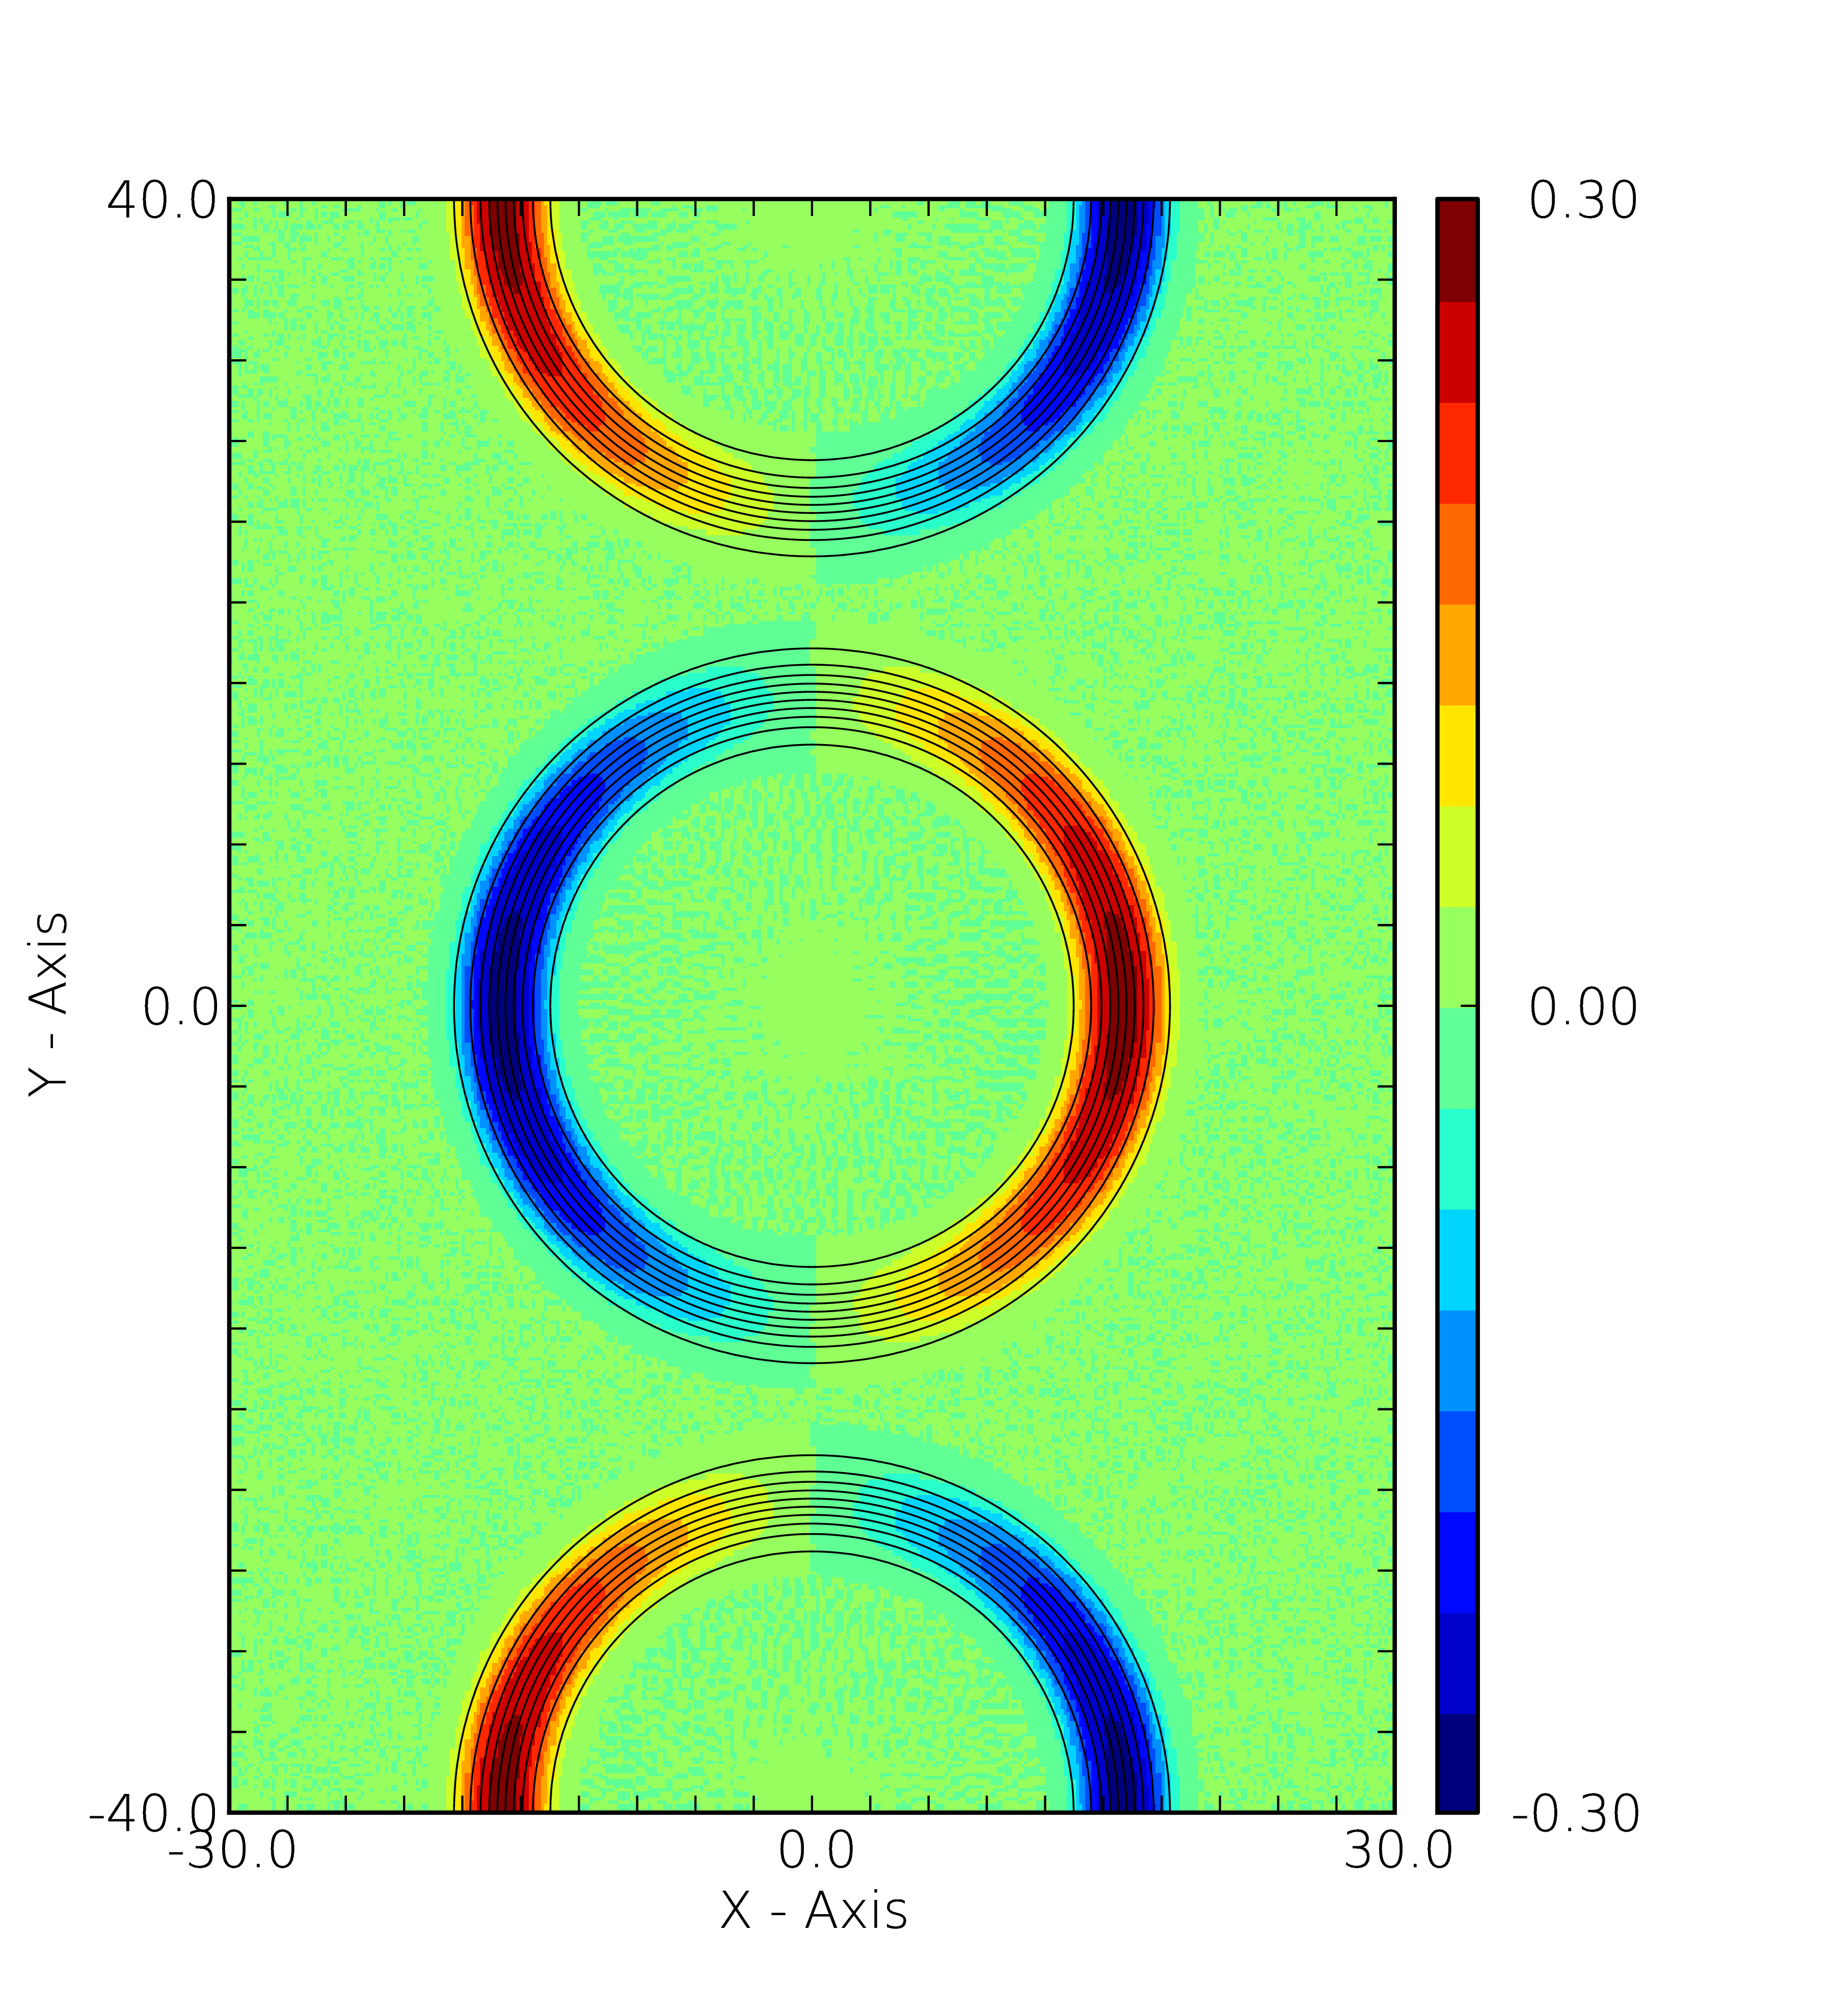
\includegraphics[width=0.6\textwidth]{bz0.jpg}
\end{center}

\end{slide}

% ____________________________________________________________________________
\begin{slide}
\large{\textbf{Non-Coplanar Hybrid simulation : t=16}}

\begin{center}
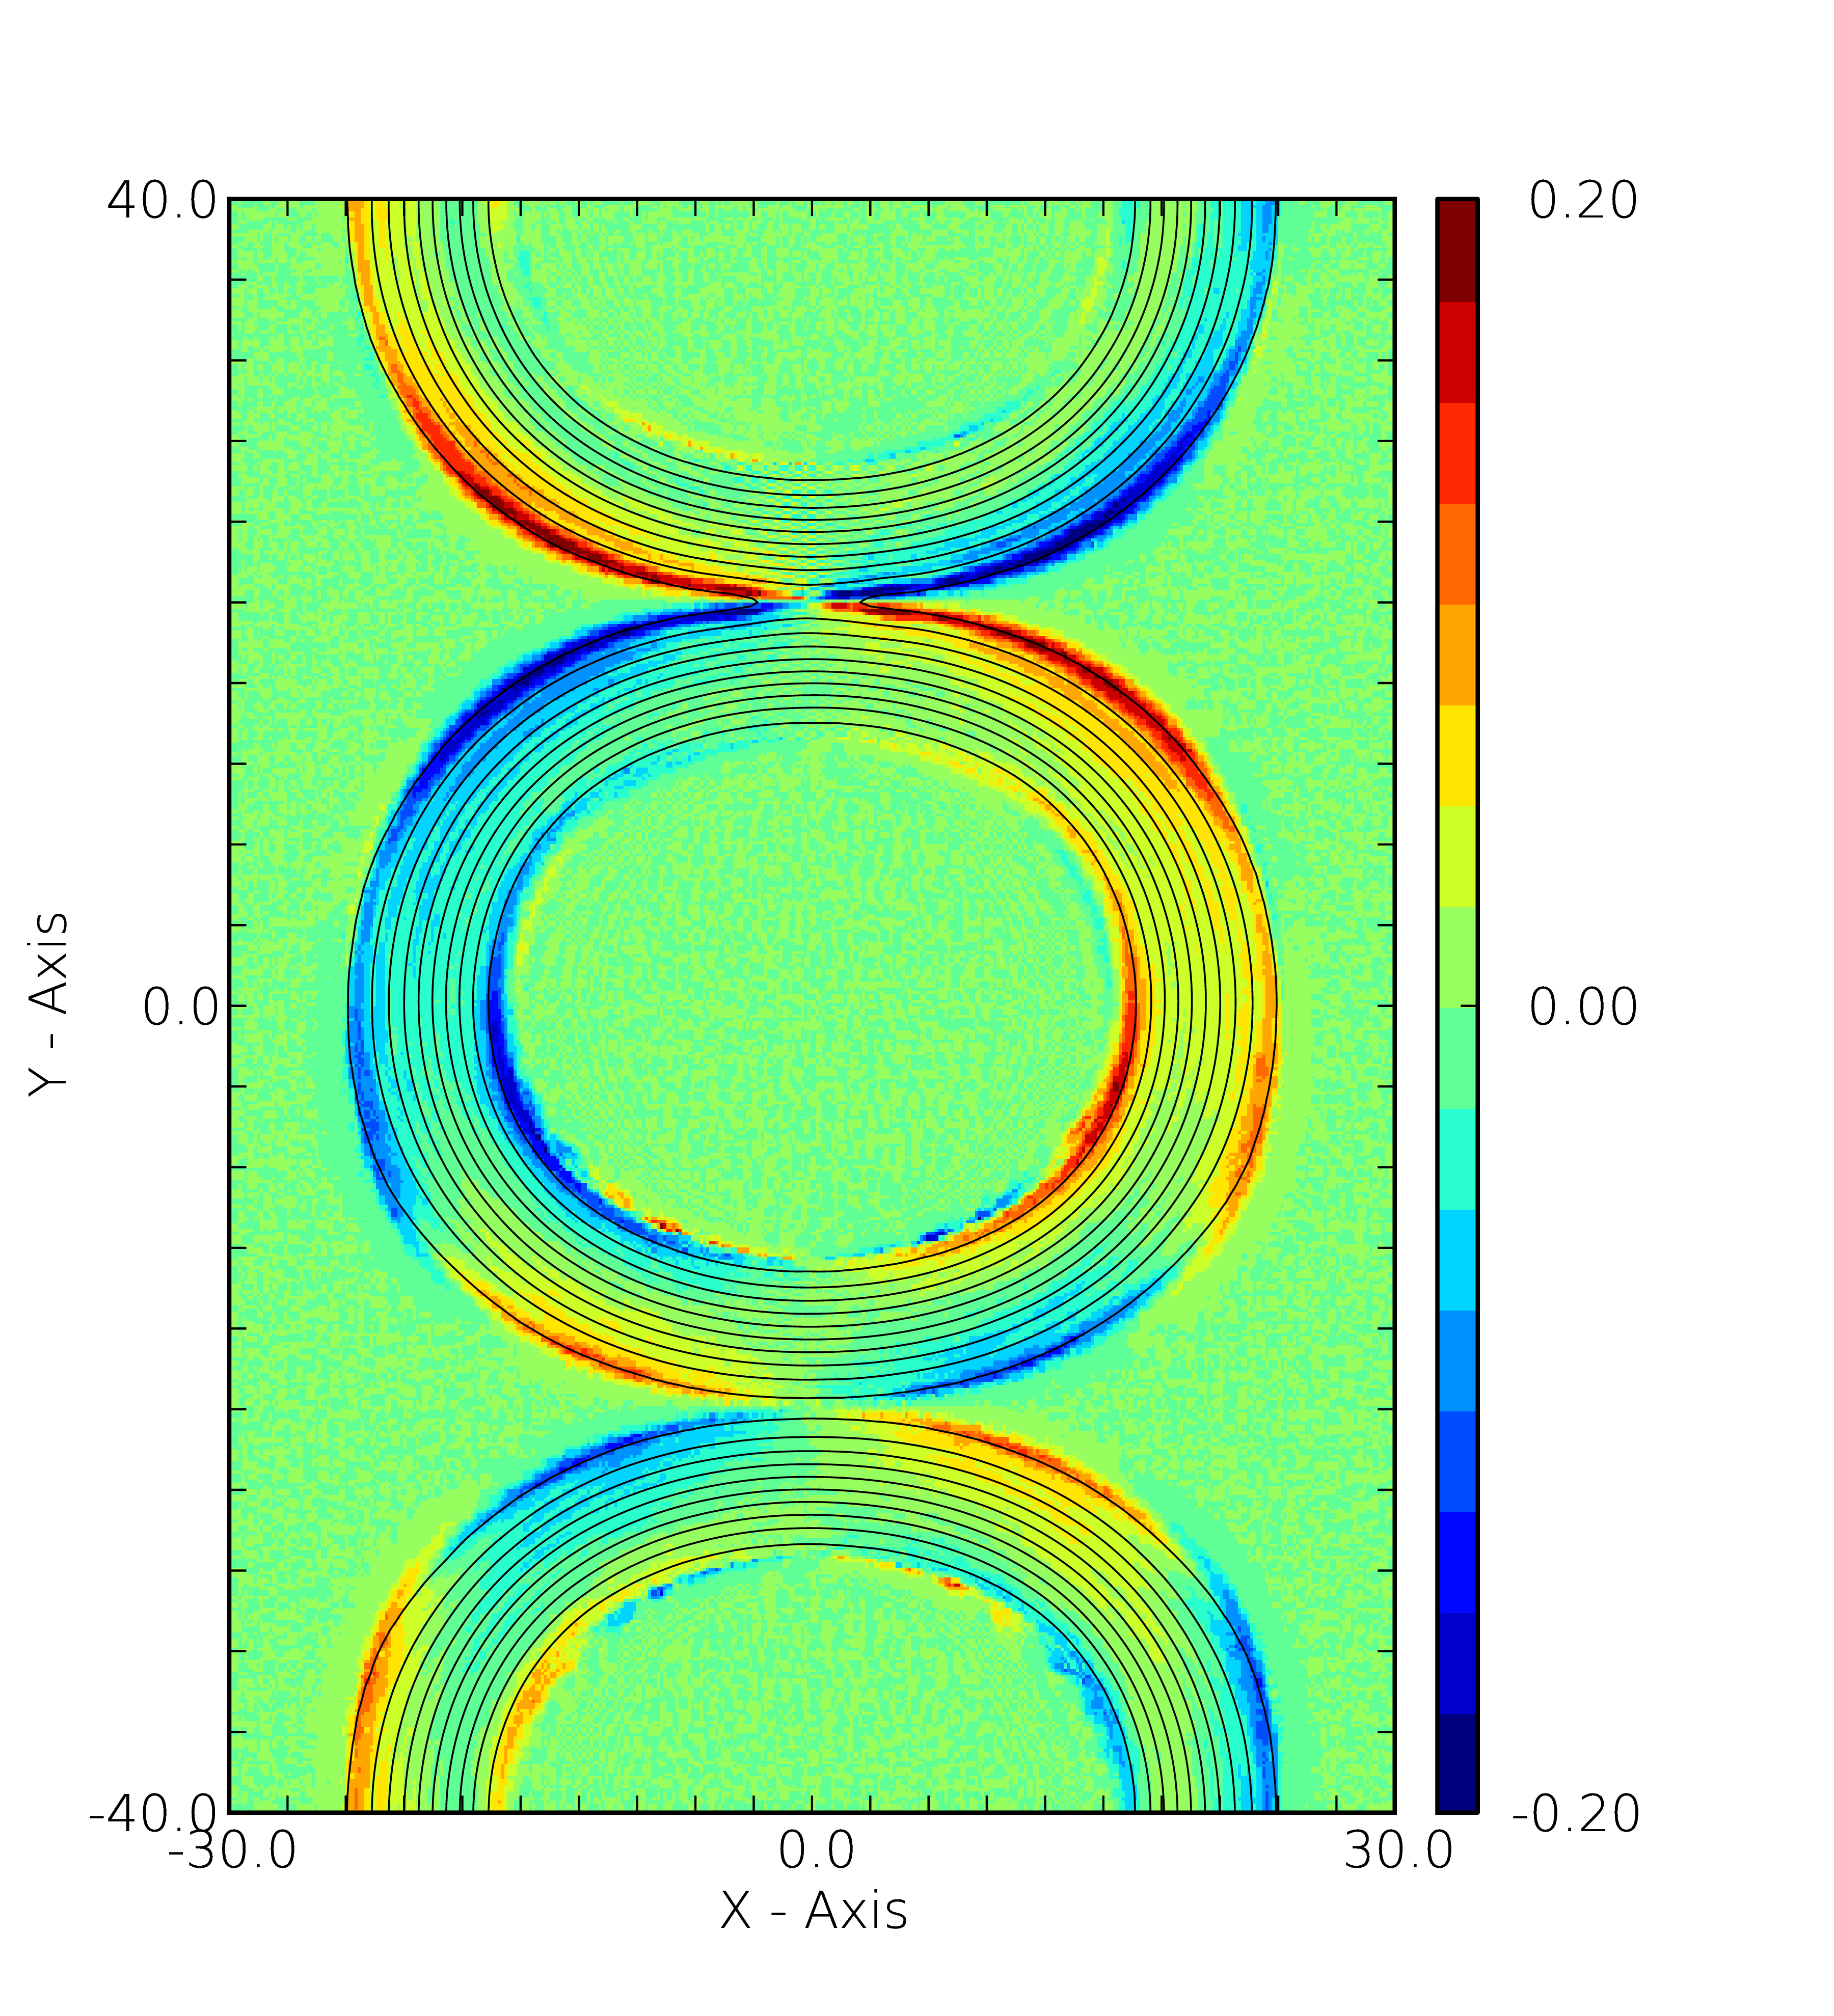
\includegraphics[width=0.6\textwidth]{bz16.jpg}
\end{center}

\end{slide}

% ____________________________________________________________________________
\begin{slide}
\large{\textbf{Main result of} [Smets et al., 2014]}

$\bullet$ A quadrupolar B field develops in thin \& compressed current sheet\\
$\bullet$ These are also the condition to trigger magnetic reconnection\\
$\rightarrow$ hence quadrupolar B field develops \underline{before} reconnection

$\bullet$ The quadrupolar B field is not a consequence of reconnection\\
$\rightarrow$ neither a cause... but "concomitant" with reconnection\\


\end{slide}

%%% % ____________________________________________________________________________
%%% \begin{slide}
%%% \large{\textbf{Reconnected flux}}
%%% 
%%% \begin{center}
%%% \includegraphics[width=0.8\textwidth]{phi01f.jpg}
%%% \end{center}
%%% 
%%% $B_Z$ develops prior the reconnection onset (t=16)\\
%%% Same reconnection rate at each loci (slope of $A_Z$)\\
%%% Time lag between the 2 onsets of reconnection
%%% 
%%% \end{slide}

%%% % ____________________________________________________________________________
%%% \begin{slide}
%%% \large{\textbf{LULI 2000 : 2 beams with 200 J \& 4.0 ns each}}
%%% 
%%% \begin{center}
%%% \includegraphics[width=0.9\textwidth]{Au-plane.png}
%%% \end{center}
%%% 
%%% $\rightarrow$ The 2 magnetic shells get compressed and get flat\\
%%% $\rightarrow$ On the reconnection sheet, protons are weakly scattered
%%% 
%%% \end{slide}

%%% % ____________________________________________________________________________
%%% \begin{slide}
%%% \large{\textbf{LULI 2000 : 2 beams with 200 J \& 4.0 ns each}}
%%% 
%%% \begin{center}
%%% \includegraphics[width=0.9\textwidth]{Au-anti.png}
%%% \end{center}
%%% 
%%% $\rightarrow$ No more flat sheet betweens the 2 shells\\
%%% $\rightarrow$ Reconnection inhibited ?
%%% 
%%% \end{slide}

% ____________________________________________________________________________
\begin{slide}
\large{\textbf{With a different folding}}

\input{_guide}

$\bullet$ Initial non-uniform Guide-field\\
$\rightarrow$ generally slows-down the (symmetrical) reconnection

\end{slide}

%%% % ____________________________________________________________________________
%%% \begin{slide}
%%% \large{\textbf{LMJ/PETAL shots end of 2017}}
%%% 
%%% $\bullet$ 800 kJ, 4 ns with 4 quads\\[0.4cm]
%%% $\bullet$ Increase magnetization \& shorten reconnection process\\[0.4cm]
%%% $\bullet$ High Z target decreases the associated $\beta$ value\\[0.4cm]
%%% $\bullet$ Proton radiography\\
%%% $\rightarrow$ Get (integrated) $E$ \& $B$ fields at different times\\[0.4cm]
%%% $\bullet$ DP1 X-ray imager : 12 images with resolution of 130 ps\\
%%% $\rightarrow$ a sequence of 2D images\\[0.4cm]
%%% $\bullet$ DMX Spectrometer : X-rays spectra resolved in time\\
%%% $\rightarrow$ measure the black-body spectrum of $T \sim$ 100 eV plasma
%%% 
%%% \end{slide}

% ____________________________________________________________________________
\begin{slide}
\large{\textbf{Experimental setup at LULI 2000 (in 2017)}}

\begin{center}
\includegraphics[width=1.0\textwidth]{manip.png}
\end{center}

\end{slide}

% ____________________________________________________________________________
\begin{slide}
\large{\textbf{Hybrid-PIC simulation for simplified 2D case}}

\begin{center}
\includegraphics[width=0.8\textwidth]{simu2D.png}
\end{center}

\end{slide}

% ____________________________________________________________________________
\begin{slide}
\large{\textbf{Synthetic RCF for 10 MeV proton beam}}

\begin{center}
\includegraphics[width=0.8\textwidth]{rcf2D.png}
\end{center}

$\rightarrow$ a "mouth" open when B field is compressed\\
$\rightarrow$ but closes when recnnection operate (and decrease B)\\

\end{slide}

% ____________________________________________________________________________
\begin{slide}
\large{\textbf{Synthetic RCF for 10 MeV proton beam}}

\begin{center}
\includegraphics[width=0.6\textwidth]{crados.png}
\end{center}

$\rightarrow$ for coplanar reconnection, no magnetic field pile-up : magnetic flux is expelled by reconnection\\
$\rightarrow$ "guided" reconnection is triggering later and/or at a smaller rate\\

\end{slide}

% ____________________________________________________________________________
\begin{slide}
\large{\textbf{Streaked Optical Pyrometry}}

\begin{center}
\includegraphics[width=0.36\textwidth]{fig2_vSOP_v5}
\end{center}

$\rightarrow$ emissivity increases with density because of the pile-up\\
$\rightarrow$ emissivity decreases for hot plasma

\end{slide}


% ____________________________________________________________________________
\begin{slide}
\large{\textbf{3D Hybrid-PIC simulations : "heated" and "feeded"}}

% $\bullet$ Including an (electron) heating and (ion) feeding operator

\begin{center}
\includegraphics[width=0.7\textwidth]{fig4}
\end{center}

%$\rightarrow$ the "in-plane" magnetic field is almost the same\\
%$\rightarrow$ the plasma weakly depends on the axial coordinate

\end{slide}


% ____________________________________________________________________________
\begin{slide}
\large{\textbf{Energy dissipation and electron heating}}

\begin{center}
\includegraphics[width=0.5\textwidth]{je_te}
\end{center}

$\rightarrow$ smaller energy dissipation for larger angles\\
$\rightarrow$ and also less efficient heating of the electrons

\end{slide}

% ____________________________________________________________________________
\begin{slide}
    \large{\textbf{Concluding remarks} : [Bolanos et al., Nat. Comm., 2022]}

$\bullet$ Magnetic reconnection becomes less efficient when increasing the tilt angle between two flux-tubes\\
$\bullet$ Experiment point that when increasing the angle between the two targets :\\
-- enhancement of the magnetic compression\\
-- larger electron density\\
-- smaller electron temperature in the current sheet

$\bullet$ 3D hybrid-PIC simulations concur with the observations\\
$\rightarrow$ drop of efficiency of the reconnection process

\end{slide}

\end{document}
